\documentclass[]{jarticle}          % 一段組
%\documentclass[twocolumn]{jarticle} % 二段組

\textwidth 180mm
\textheight 255mm
\oddsidemargin -12mm
\topmargin -15mm
\columnsep 10mm

%\vspace{0.5cm} % 一段組の場合はコメントアウトした方が体裁がよいx
%] % 一段組の場合はコメントアウトする

\usepackage{styles/labheadings}
\usepackage[dvipdfmx]{graphicx,color}
\usepackage{amsmath,amssymb}
\usepackage{url}
% 追加
\usepackage{listings,jvlisting}
\usepackage[hang,small,bf]{caption}
\usepackage[subrefformat=parens]{subcaption}
\captionsetup{compatibility=false}

\newcommand{\aU}{\mbox{\boldmath $a$}}
\newcommand{\bU}{\mbox{\boldmath $b$}}
\newcommand{\cU}{\mbox{\boldmath $c$}}
\newcommand{\dU}{\mbox{\boldmath $d$}}
\newcommand{\eU}{\mbox{\boldmath $e$}}
\newcommand{\fU}{\mbox{\boldmath $f$}}
\newcommand{\gU}{\mbox{\boldmath $g$}}
\newcommand{\hU}{\mbox{\boldmath $h$}}
\newcommand{\iU}{\mbox{\boldmath $i$}}
\newcommand{\jU}{\mbox{\boldmath $j$}}
\newcommand{\kU}{\mbox{\boldmath $k$}}
\newcommand{\lU}{\mbox{\boldmath $l$}}
\newcommand{\mU}{\mbox{\boldmath $m$}}
\newcommand{\nU}{\mbox{\boldmath $n$}}
\newcommand{\oU}{\mbox{\boldmath $o$}}
\newcommand{\pU}{\mbox{\boldmath $p$}}
\newcommand{\qU}{\mbox{\boldmath $q$}}
\newcommand{\rU}{\mbox{\boldmath $r$}}
\newcommand{\sU}{\mbox{\boldmath $s$}}
\newcommand{\tU}{\mbox{\boldmath $t$}}
\newcommand{\uU}{\mbox{\boldmath $u$}}
\newcommand{\vU}{\mbox{\boldmath $v$}}
\newcommand{\wU}{\mbox{\boldmath $w$}}
\newcommand{\xU}{\mbox{\boldmath $x$}}
\newcommand{\yU}{\mbox{\boldmath $y$}}
\newcommand{\zU}{\mbox{\boldmath $z$}}
\newcommand{\AU}{\mbox{\boldmath $A$}}
\newcommand{\BU}{\mbox{\boldmath $B$}}
\newcommand{\CU}{\mbox{\boldmath $C$}}
\newcommand{\DU}{\mbox{\boldmath $D$}}
\newcommand{\EU}{\mbox{\boldmath $E$}}
\newcommand{\FU}{\mbox{\boldmath $F$}}
\newcommand{\GU}{\mbox{\boldmath $G$}}
\newcommand{\HU}{\mbox{\boldmath $H$}}
\newcommand{\IU}{\mbox{\boldmath $I$}}
\newcommand{\JU}{\mbox{\boldmath $J$}}
\newcommand{\KU}{\mbox{\boldmath $K$}}
\newcommand{\LU}{\mbox{\boldmath $L$}}
\newcommand{\MU}{\mbox{\boldmath $M$}}
\newcommand{\NU}{\mbox{\boldmath $N$}}
\newcommand{\OU}{\mbox{\boldmath $O$}}
\newcommand{\PU}{\mbox{\boldmath $P$}}
\newcommand{\QU}{\mbox{\boldmath $Q$}}
\newcommand{\RU}{\mbox{\boldmath $R$}}
\newcommand{\SU}{\mbox{\boldmath $S$}}
\newcommand{\TU}{\mbox{\boldmath $T$}}
\newcommand{\UU}{\mbox{\boldmath $U$}}
\newcommand{\VU}{\mbox{\boldmath $V$}}
\newcommand{\WU}{\mbox{\boldmath $W$}}
\newcommand{\XU}{\mbox{\boldmath $X$}}
\newcommand{\YU}{\mbox{\boldmath $Y$}}
\newcommand{\ZU}{\mbox{\boldmath $Z$}}
\newcommand{\epU}{\mbox{\boldmath $\epsilon$}}
\newcommand{\taU}{\mbox{\boldmath $\tau$}}
\newcommand{\etU}{\mbox{\boldmath $\eta$}}
\newcommand{\xiU}{\mbox{\boldmath $\xi$}}
\newcommand{\wwU}{\mbox{\boldmath $\omega$}}
\newcommand{\WwU}{\mbox{\boldmath $\Omega$}}
\newcommand{\lmU}{\mbox{\boldmath $\lambda$}}
\newcommand{\LmU}{\mbox{\boldmath $\Lambda$}}
\newcommand{\PiU}{\mbox{\boldmath $\Pi$}}
\newcommand{\SgU}{\mbox{\boldmath $\Sigma$}}
\newcommand{\thU}{\mbox{\boldmath $\theta$}}
\newcommand{\ThU}{\mbox{\boldmath $\Theta$}}
\newcommand{\roU}{\mbox{\boldmath $\rho$}}
\newcommand{\nuU}{\mbox{\boldmath $\nu$}}
\newcommand{\ones}{{\bf 1}}
\newcommand{\zr}{{\bf 0}}
\newcommand{\eq}{\begin{equation}}
\newcommand{\en}{\end{equation}}
\newcommand{\eqa}{\begin{eqnarray}}
\newcommand{\ena}{\end{eqnarray}}
\newcommand{\xx}{\makebox[1cm]{}}
\newcommand{\xm}{\makebox[0.5cm]{}}
\newcommand{\x}{\makebox[0.2cm]{}}
\newcommand{\tr}{{\rm tr}}
\newcommand{\sgn}{{\rm sgn}}
\newcommand{\ad}{{\rm ad}}

\newcommand{\rank}{{\rm rank}}
\newcommand{\diag}{{\rm diag}}
\newcommand{\lbr}{\left(\begin{array}}
\newcommand{\rbr}{\end{array}\right)}
\newcommand{\Proof}{\noindent{\em Proof\/}}
\newcommand{\Solution}{\noindent{\em Solution}}
\newcommand{\Derivation}{\noindent{\em Derivation}}
\newcommand{\msp}{\vspace*{\medskipamount}\\}
\newcommand{\qed}{\hspace*{\fill}$\Box$}
\newcommand{\aX}{{\bf a}}
\newcommand{\bX}{{\bf b}}
\newcommand{\cX}{{\bf c}}
\newcommand{\dX}{{\bf d}}
\newcommand{\eX}{{\bf e}}
\newcommand{\fX}{{\bf f}}
\newcommand{\gX}{{\bf g}}
\newcommand{\hX}{{\bf h}}
\newcommand{\iX}{{\bf i}}
\newcommand{\jX}{{\bf j}}
\newcommand{\kX}{{\bf k}}
\newcommand{\lX}{{\bf l}}
\newcommand{\mX}{{\bf m}}
\newcommand{\nX}{{\bf n}}
\newcommand{\oX}{{\bf o}}
\newcommand{\pX}{{\bf p}}
\newcommand{\qX}{{\bf q}}
\newcommand{\rX}{{\bf r}}
\newcommand{\sX}{{\bf s}}
\newcommand{\tX}{{\bf t}}
\newcommand{\uX}{{\bf u}}
\newcommand{\vX}{{\bf v}}
\newcommand{\wX}{{\bf w}}
\newcommand{\xX}{{\bf x}}
\newcommand{\yX}{{\bf y}}
\newcommand{\zX}{{\bf z}}
\newcommand{\AX}{{\bf A}}
\newcommand{\BX}{{\bf B}}
\newcommand{\CX}{{\bf C}}
\newcommand{\DX}{{\bf D}}
\newcommand{\EX}{{\bf E}}
\newcommand{\FX}{{\bf F}}
\newcommand{\GX}{{\bf G}}
\newcommand{\HX}{{\bf H}}
\newcommand{\IX}{{\bf I}}
\newcommand{\JX}{{\bf J}}
\newcommand{\KX}{{\bf K}}
\newcommand{\LX}{{\bf L}}
\newcommand{\MX}{{\bf M}}
\newcommand{\NX}{{\bf N}}
\newcommand{\OX}{{\bf O}}
\newcommand{\PX}{{\bf P}}
\newcommand{\QX}{{\bf Q}}
\newcommand{\RX}{{\bf R}}
\newcommand{\SX}{{\bf S}}
\newcommand{\TX}{{\bf T}}
\newcommand{\UX}{{\bf U}}
\newcommand{\VX}{{\bf V}}
\newcommand{\WX}{{\bf W}}
\newcommand{\XX}{{\bf X}}
\newcommand{\YX}{{\bf Y}}
\newcommand{\ZX}{{\bf Z}}

% report.texと同じディレクトリにnumerical_definition.texを入れておけば上の書き方でもいいはずです

\usepackage[
  dvipdfm,
  bookmarks=true,
  bookmarksnumbered=true,
  colorlinks=true]{hyperref}
\AtBeginDvi{\special{pdf:tounicode EUC-UCS2}}

%ここからソースコードの表示に関する設定
\lstset{
  basicstyle={\ttfamily},
  identifierstyle={\small},
  commentstyle={\smallitshape},
  keywordstyle={\small\bfseries},
  ndkeywordstyle={\small},
  stringstyle={\small\ttfamily},
  frame={tb},
  breaklines=true,
  columns=[l]{fullflexible},
  numbers=left,
  xrightmargin=0zw,
  xleftmargin=3zw,
  numberstyle={\scriptsize},
  stepnumber=1,
  numbersep=1zw,
  lineskip=-0.5ex
}
%ここまでソースコードの表示に関する設定

\pagestyle{labheadings}
\headerleft{進捗報告}   % ヘッダの左側のタイトル
\headerright{2023年06月16日}  % ヘッダの右側のタイトル

\begin{document}

%\twocolumn % 一段組の場合はコメントアウトする

\vspace*{2ex}
\begin{center}
 {\Large \bf 三次元モデル作成と顔の特徴点座標抽出}\\ % タイトル
 \vspace*{5mm}
 {\large B4 田川幸汰}% 発表者名
\end{center}

%\vspace{0.5cm} % 一段組の場合はコメントアウトした方が体裁がよいx
%] % 一段組の場合はコメントアウトする

%新しく作成したコマンド
% \newcommand{\reffig}[1]{\hyperref[#1]{図\ref{#1}}}
% \newcommand{\refeq}[1]{\hyperref[#1]{式(\ref{#1})}}
% \newcommand{\reftab}[1]{\hyperref[#1]{表\ref{#1}}}
% \newcommand{\refsec}[1]{\hyperref[#1]{\ref{#1}章}}
% \newcommand{\refsubsec}[1]{\hyperref[#1]{\ref{#1}節}}

% 数式

% 図
% \begin{figure}[!ht]
%   \begin{center}
%     \includegraphics[scale=0.5]{figures/画像ファイル名}
%     \caption{キャプション名}
%     \label{ラベル名}
%   \end{center}
% \end{figure}

% リスト
% \begin{enumerate or itemize}
%   \item 
% \end{enumerate or itemize}

\section{概要}
 進捗報告として三次元モデルの作成と顔の特徴点座標抽出を発表する。 \\
 三次元モデルの作成、顔の特徴点抽出を達成するために用いた技術と、その結果を以下の章で説明する。

\section{三次元モデルの作成}
三次元モデルをBlenderのアドオンであるFaceBuilderを用いて作成した。
\subsection{FaceBuilder}
FaceBuilderは、人間の顔や頭部のモデリングを簡単に行うためのツールである。
FaceBuilderを使用すると、写真やビデオから自動的に顔のモデルを作成することができる。
また顔の形状や解像度の詳細な調整、テクスチャの適用など、モデルのカスタマイズもサポートしている。
他のBlenderの機能とも連携し、リグやアニメーションの作成など、さまざまな作業を補助することができる。
FaceBuilderは以下のように使う。
\begin{enumerate}
  \item FaceBuilderのタブから[Create new head]を選択
  \item 下絵となる写真を一枚以上[Add Images]より追加
  \item openした画像を選択して[Align face]を選択
  \item 顔のラインに合わせてメッシュを微調整し[Create texture]を選択
  \item 様々な3次元、2次元形式でモデルやテクスチャをエクスポートする
\end{enumerate}

\subsection{実行結果}
\subsubsection{入力画像}
入力として、今回は\hyperref[one]{図\ref{one}}の1枚の画像を用いた。
\begin{figure}[!ht]
  \begin{center}
    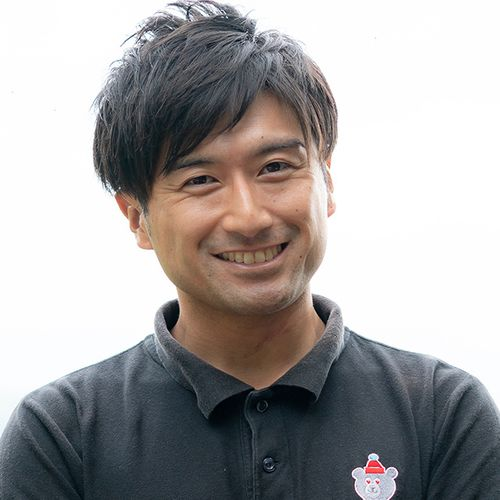
\includegraphics[scale=0.3]{figures/man1.jpg}
    \caption{入力画像}
    \label{one}
  \end{center}
\end{figure}
\subsubsection{出力画像}
出力された3次元モデルは\hyperref[two]{図\ref{two}}である。
正面はきれいにテクスチャが貼られているが、側面、裏面は画像に写っていないので貼られていない。
複数枚の写真を用いて側面を描画することも可能であるが、顔の正面に写るマスク部分の描画であれば、顔画像一枚でも問題ないと考える。
\begin{figure}[!ht]
  \begin{center}
    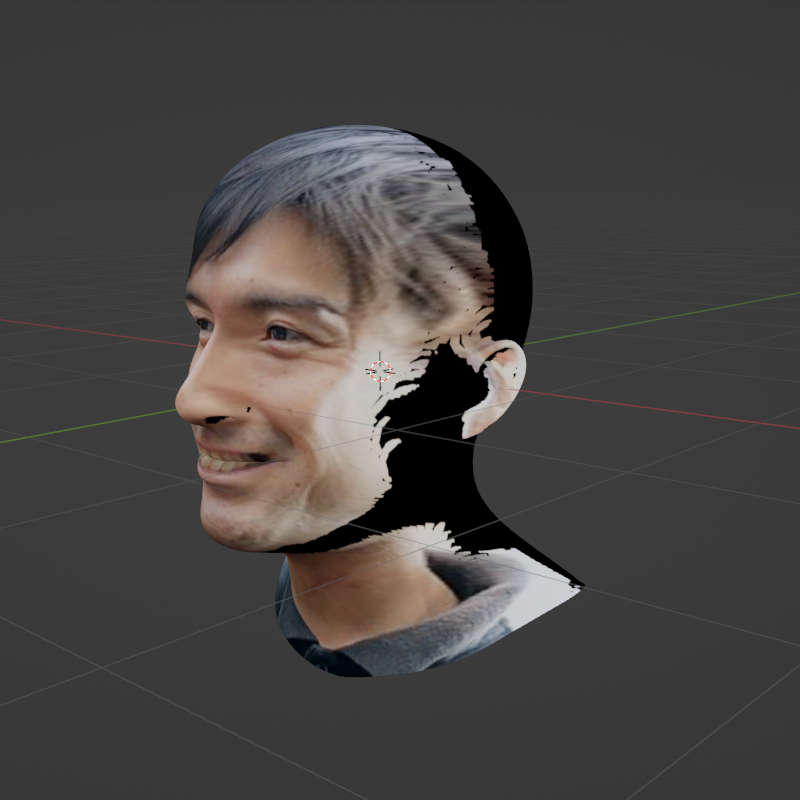
\includegraphics[scale=0.25]{figures/man3d.png}
    \caption{出力画像}
    \label{two}
  \end{center}
\end{figure}

\subsubsection{頂点座標の出力}
blenderのテキストエディタでpythonコードを記述し、作成した3次元モデルの頂点座標を出力する。
\hyperref[three]{図\ref{three}}はblenderの3dビューを表した図である。
lenderの3dビューはシーン、コレクション、オブジェクトといったように階層化されている特徴がある。
pythonのbpyライブラリを用いることで、3次元モデルのメッシュ情報にアクセスできる。
メッシュ情報には大量の頂点座標がベクトル形式で記述されている。
% 図を作る
\begin{figure}[!ht]
  \begin{center}
    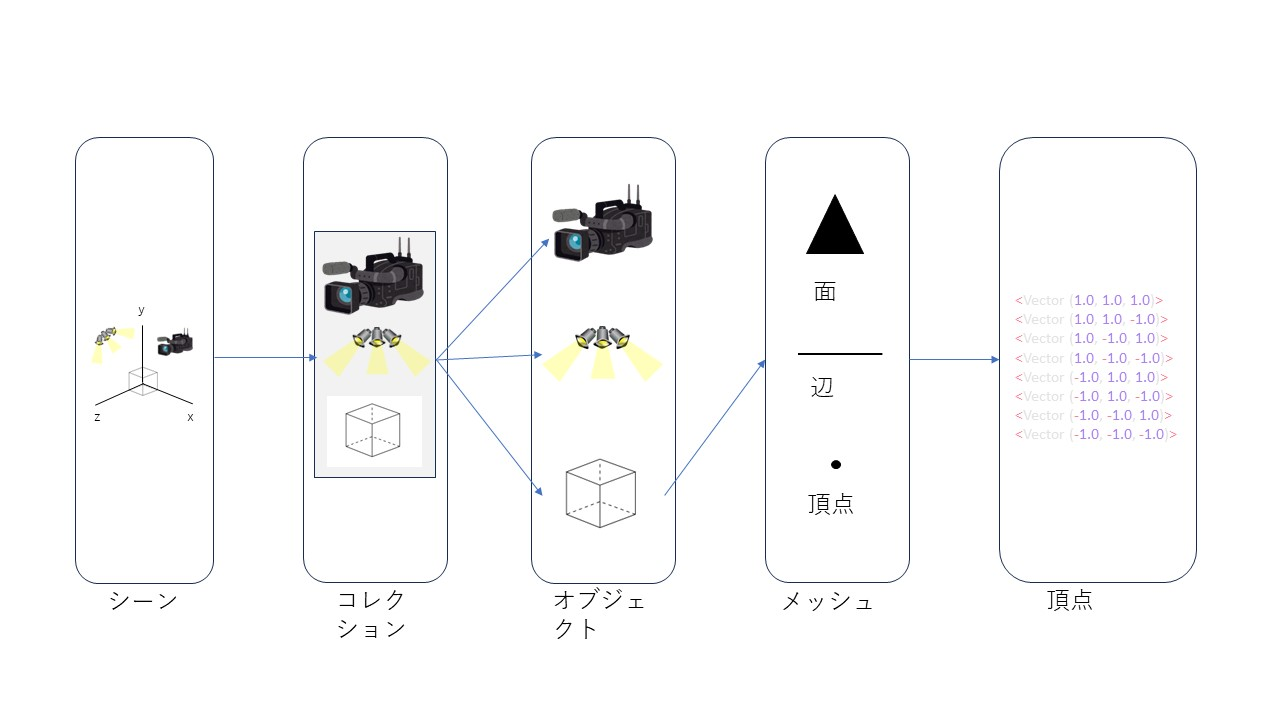
\includegraphics[scale=0.5]{figures/blender.jpg}
    \caption{blenderの3dビューのイメージ}
    \label{three}
  \end{center}
\end{figure}

\hyperref[four]{図\ref{four}}は実際に出力された頂点座標を、pythonのmatplotlibライブラリを用いて3次元座標空間に出力した図である。
\begin{figure}[!ht]
  \begin{center}
    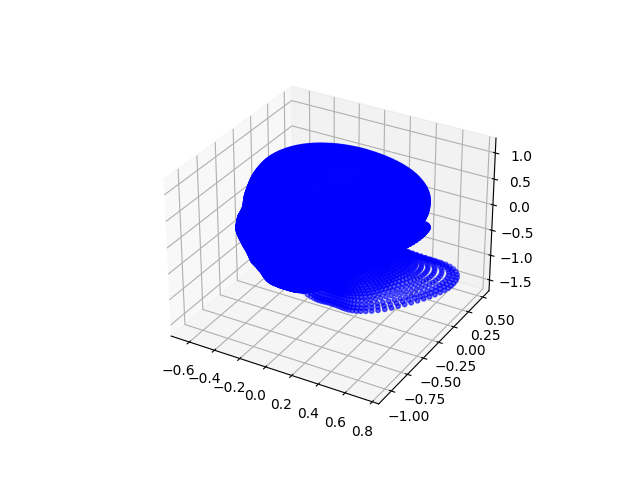
\includegraphics[scale=0.7]{figures/coord530.png}
    \caption{頂点座標}
    \label{four}
  \end{center}
\end{figure}
なお、頂点座標は$X$,$Y$,$Z$軸ともに正規化は行われていない。


\section{顔の特徴点抽出}
Google MediapipeのFaceMeshの機能を用いて、顔の画像からフェイスメッシュを作成する。
\subsection{FaceMesh}
Googleが開発したリアルタイムの顔のマーキングシステムである。
FaceMeshは、ビデオやWebカメラの入力から、顔の輪郭、目、鼻、口などのさまざまな顔の特徴点を検出することができる。
また、深層学習モデルに基づいており、ニューラルネットワークを使用して顔の特徴点を予測する。
入力画像またはビデオフレームをFaceMeshに渡すと、顔の特徴点の3D座標と2D画像上の位置を返す。
これにより、顔の構造や表情の解析、AR(拡張現実)アプリケーションの開発などに応用される。

\subsection{実行結果}
\hyperref[five]{図\ref{five}}にFaceMeshを実行した画像を示す。このように顔上の特徴点を得ることができている。
\begin{figure}[!ht]
  \begin{center}
    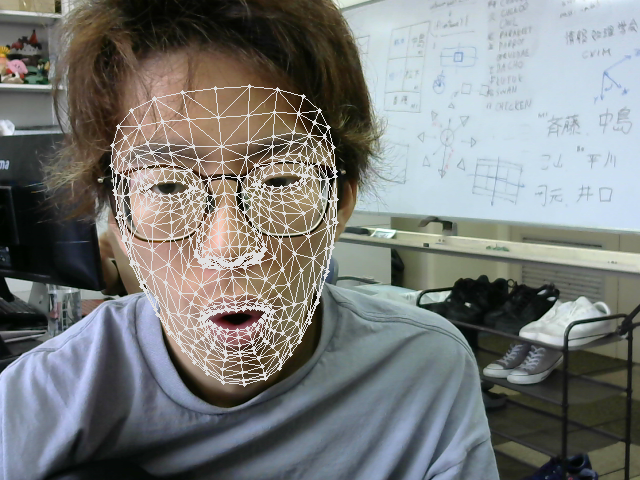
\includegraphics[scale=0.35]{figures/facemesh.png}
    \caption{facemesh}
    \label{five}
  \end{center}
\end{figure}
また、座標点を取得することもできる。なお$X$,$Y$,$Z$軸は正規化されていることに気をつけなければならない。

\subsection{顔の特徴点を基に3次元モデルを張り付け}
PythonのOpenGLライブラリを用いて、Facemeshで得られた顔の特徴点から三次元モデルを張り付けた。
\subsubsection{OpenGL}
OpenGL(Open Graphics Library)は、2Dおよび3Dグラフィックスを描画するためのクロスプラットフォームなグラフィックスAPIで、
OpenGLは、コンピュータ上でリアルタイムのグラフィックス処理を行うための一連の関数と命令のセットである。
これらの関数を使用して、点、線、三角形などのプリミティブ(基本図形)を描画し、テクスチャを貼り付け、光源やマテリアルの効果を適用することができる。

\subsubsection{グラフィックス処理}
OpenGLで用いた様々なグラフィックス処理と、それに用いた関数を下に記述する。\\
\indent 射影変換行列...カメラ座標系に計算された行列を、OpenGLのウィンドウが映し出すスクリーン座標系に変換するための行列。平行投影変換と、透視投影変換に分けられる。
透視投影変換を行うことで、カメラで写された範囲をどの程度の範囲で、どこまで見ることができるかという問題を解決する。
glMatrixMode(GL\_PROJECTION)で射影行列を選択し、glFrustum()で透視変換行列を作成。\\
\indent モデルビュー行列...物体が存在する世界座標系を、その物体を見ている視点であるカメラ座標系に変換するための行列。
視界変換と、モデリング変換からなるが、これは同一の処理を行うことを指すため、モデルビューとして一括される。
glMatrixMode(GL\_MODELVIEW)でモデルビュー行列を選択し、glLoadMatrixf()で作成。\\
\indent 光の設定...OpenGLでは光を演出するために光源と反射を処理することができる。glLightfv()でパラメータを設定。
glEnable(GL\_LIGHTING)で光源を有効にする。\\
\indent カメラ位置の設定...オブジェクトの二次元座標と三次元座標を求めることで、カメラの姿勢、姿勢を特定することができる。
これをPnP問題という。solvepnp()はPnP問題を解く関数であり、オブジェクトの二次元座標と三次元座標を引数に取り、カメラの回転ベクトル、並進ベクトルを返す。\\

\subsubsection{実行結果}
\hyperref[six]{図\ref{six}}に実行した画像を示す。このように顔上の特徴点と3次元オブジェクトを表示ことができている。
\begin{figure}[!ht]
  \begin{center}
    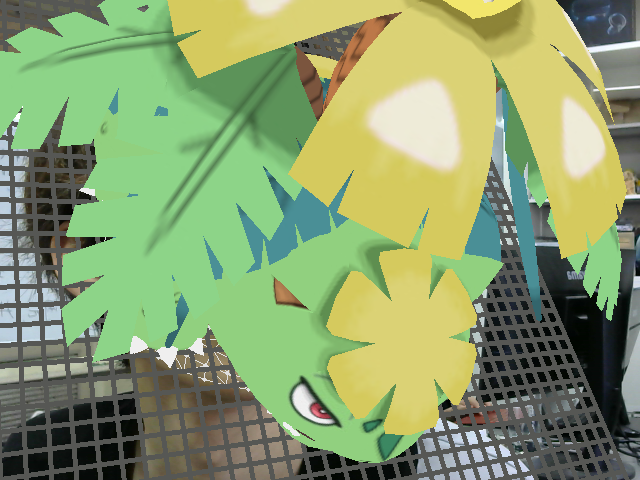
\includegraphics[scale=0.35]{figures/6.png}
    \caption{facemeshと3次元オブジェクト}
    \label{six}
  \end{center}
\end{figure}
\section{研究計画}
現時点で進行中の研究や、次回の発表時までに勧めたい研究計画を以下にまとめる。\\
\\
進行中
\begin{itemize}
  \item マスクの有無による顔上の特徴点の検出の違い
  \item mqo形式の3次元顔モデルをFaceMesh上の特徴点に合わせて貼り付け(モデルとfacemeshの座標合わせ)
\end{itemize}
次週以降
\begin{itemize}
  \item 顔上の特徴点を用いた類似研究の論文の査読
  \item 3次元顔モデルの貼り付けの修正
  \item facemeshの$Z$軸がどのように正規化されているか調べる
\end{itemize}

%参考文献
\begin{thebibliography}{99}
\bibitem{bib_1} OpenGL入門,http://wisdom.sakura.ne.jp/system/opengl/index.html,閲覧日2023/6/16
\end{thebibliography}

\end{document}
